\documentclass{beamer}

\usetheme{JuanLesPins}
\usecolortheme{seahorse}

%\useoutertheme[]{sidebar}

\setbeamercovered{transparent}

\usepackage[slovak]{babel}
\usepackage[T1]{fontenc}
\usepackage[utf8]{inputenc}
\usepackage{url}
\usepackage{listings, lstautogobble}

\def\BibTeX{\textsc{Bib}\kern-.08em\TeX} 

\definecolor{RoyalBlue}{cmyk}{1, 0.50, 0, 0}
\lstset{language=Java,
    keywordstyle=\color{RoyalBlue},
    basicstyle=\scriptsize\ttfamily,
    commentstyle=\ttfamily\itshape\color{gray},
    stringstyle=\ttfamily,
    showstringspaces=false,
    breaklines=true,
    frameround=ffff,
    rulecolor=\color{black},
    autogobble=true,
}

\newcommand{\footcite}[1]{\footnote{\tiny #1}}
\newcommand{\umlet}{.5}
\newcommand{\emp}[1]{\textit{\alert{#1}}}
\newcommand{\kw}[1]{\mbox{\textbf{#1}}}
\newcommand{\id}[1]{\texttt{#1}}
\newcommand{\stl}{\guillemotleft}
\newcommand{\str}{\guillemotright}

\setbeamertemplate{footline}[page number]

\author{Lukáš Častven}
\institute{
	Fakulta informatiky a informačných technológií\\
	Slovenská technická univerzita v Bratislave}

\subtitle{\vspace{3mm} Metódy inžinierskej práce 2020/2021}

\title{Využitie statickej analýzy kódu pri vývoji softvéru}

\date{\footnotesize 28. november 2021}


\begin{document}

% titulny slajd
\begin{frame}[fragile=singleslide]
	\titlepage
\end{frame}

% slajd s motivaciou vyberu tejto temy
\begin{frame}[fragile=singleslide]\frametitle{Motivácia}
	\begin{itemize}
		\item Spôsob udržania kvality kódu
		\item Zautomatizované hľadanie chýb a defektov
		\item \emph{,,Hoci čo, čo zautomatizuje nudnú prácu je skvele.''}~\footcite{B. Johnson, Why don't software developers use
			      staticanalysis tools to find bugs?,” IEEE, may 2013. }
	\end{itemize}
\end{frame}

% slajd s prehladom o sekciach
\begin{frame}[fragile=singleslide]\frametitle{Prehľad}
	\tableofcontents
\end{frame}


\section{Principy statickej analýzy}

\begin{frame}[fragile=singleslide]\frametitle{Principy statickej analýzy}
	\begin{itemize}
		\item Analyzovanie kódu bez spušťanie
		\item Informovanie o chybách a defektoch
		\item Príklad chybného kódu~\footcite{N. Ayewah, Using static analysis to find bugs}
		      \begin{lstlisting}
				public String founType() {
					return this.foundType();
				}
				\end{lstlisting}
	\end{itemize}
\end{frame}



\section{Využitie pri vyvoji softveru}

\begin{frame}[fragile=singleslide]\frametitle{Využitie pri vyvoji softveru}

	\begin{table}
		\begin{center}
			\begin{tabular}{l|l}
				$Benefity$                & $Nedostatky$                       \\
				\hline
				Automatické hľadanie chýb & Falošné pozitíva                   \\
				Urdžanie kvality kódu     & Prerušenie pracovného priebehu     \\
				Predintegrácia            & Nejasnosť                          \\
				Urdžanie tímových praktík & Nedostatočná podpora tímovej práce \\
				Nastaviteľnosť            & Netriviálnosť                      \\
			\end{tabular}
		\end{center}
	\end{table}

\end{frame}

\section{Implementácia nástrojov statickej analýzy}

\begin{frame}[fragile=singleslide]\frametitle{Implementácia nástrojov statickej analýzy}
	\begin{itemize}
		\item Integrované v IDE
		\item Integrované v kompilátoroch~\footcite{\url{https://developers.redhat.com/blog/2020/03/26/static-analysis-in-gcc-10\#diagnostic_paths}}
		      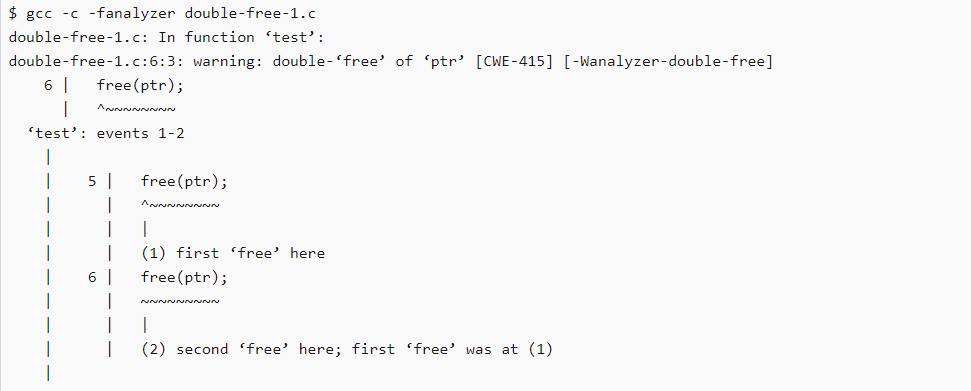
\includegraphics[scale=0.35]{SAkompiler.png}
		\item Rigorózne analyzátory
	\end{itemize}
\end{frame}

\section{Využitie v praxi}

\begin{frame}[fragile=singleslide]\frametitle{Využitie v praxi}
	\centerline{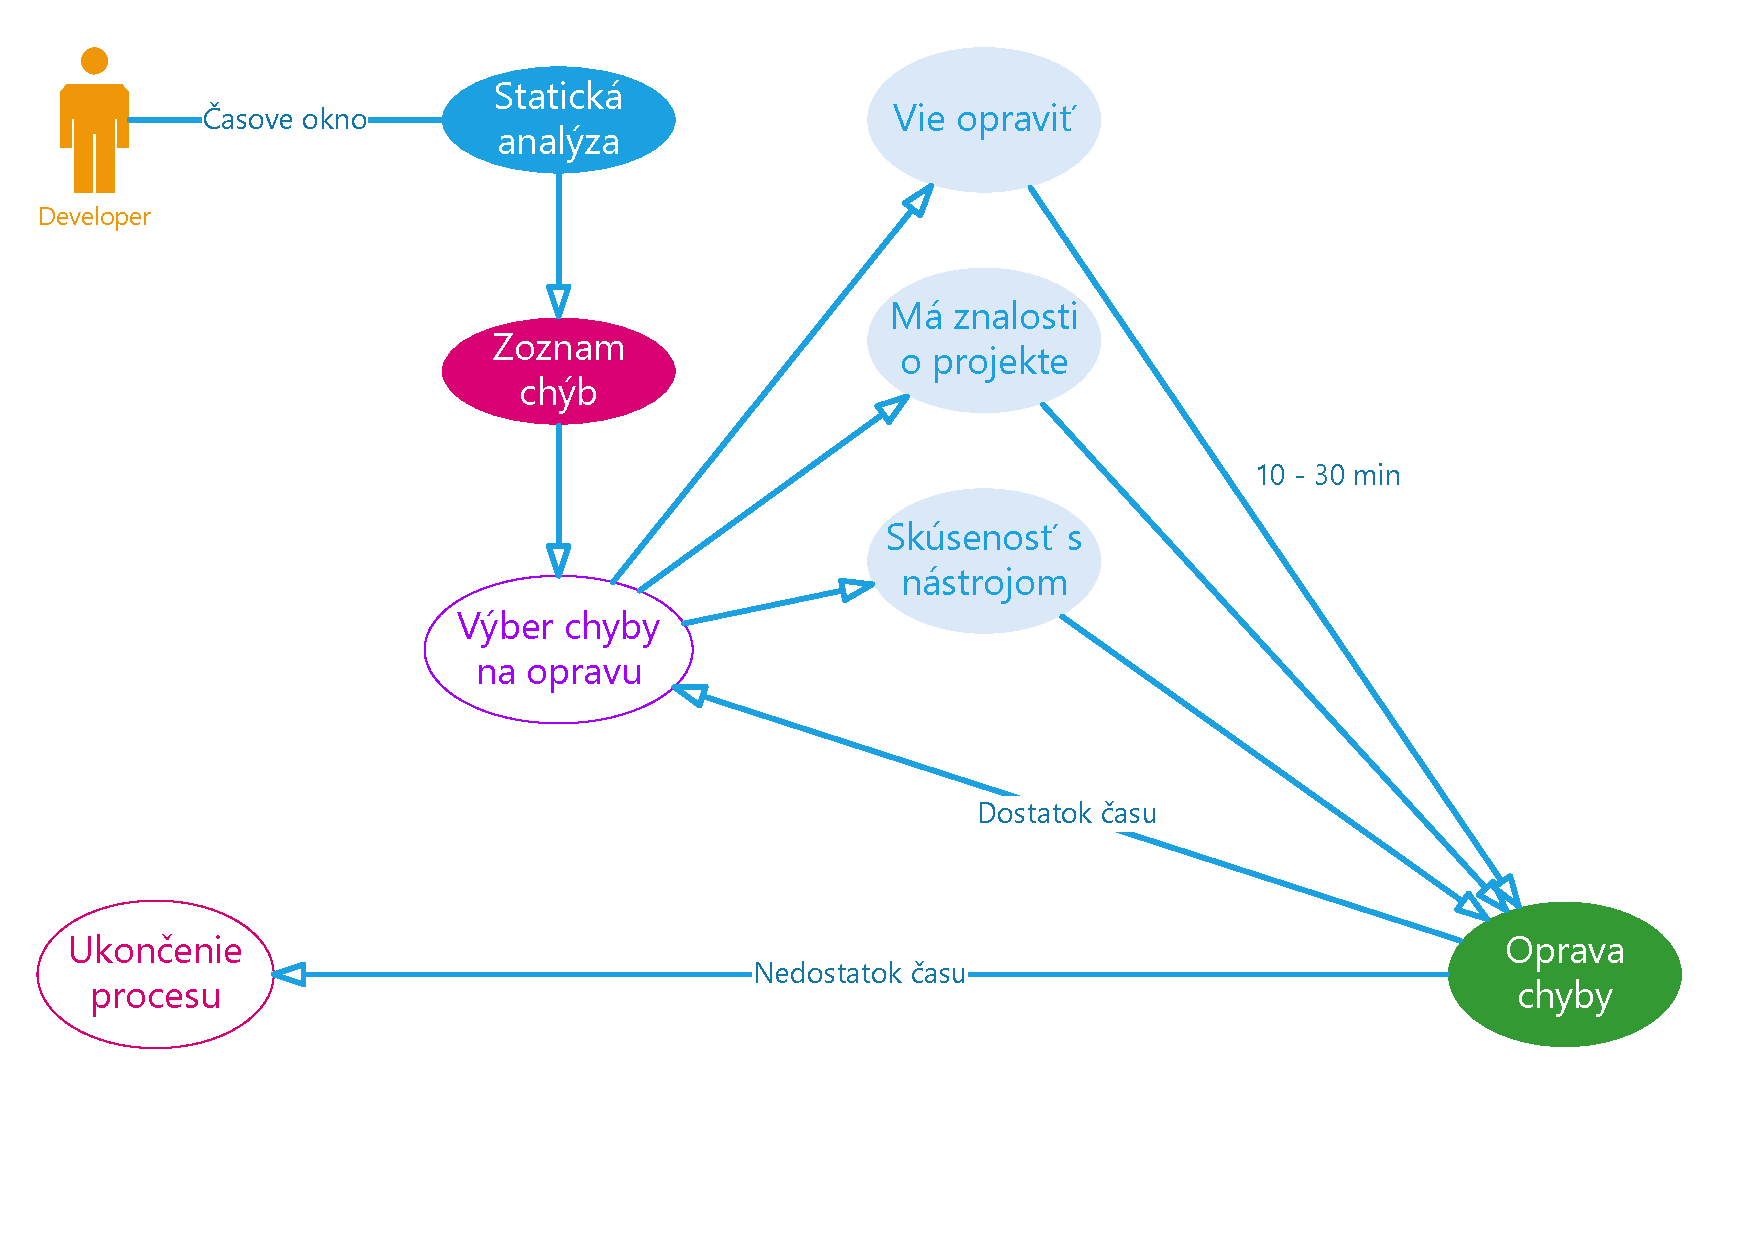
\includegraphics[scale=0.38]{vyuzitie.pdf}}
\end{frame}


\section*{Zhodnotenie a ďalšia práca}
% hviezdička zabezpečí, aby sa táto časť neocitla v prehľade prezentácie - každá prezentácia má zhodnotenie a prehľad by sa tým zbytočne zahlcoval

\begin{frame}[fragile=singleslide]\frametitle{Zhodnotenie a ďalšia práca}
	\begin{itemize}
		\item Každá prezentácia musí byť nejako uzavretá
		\item Ale vždy je čo robiť ďalej\ldots{}
	\end{itemize}
\end{frame}


\end{document}


Text \end{document} za príkazom \end{document} LaTeX ignoruje, takže tu môžete odkladať veci (aj celé slajdy), ktoré nechcete vymazať, lebo ich ešte možno budete potrebovať, avšak ich v danom momente nechcete mať v slajdoch.
